\newpage


\section{Ergebnisreflexion}
\label{ergebnisreflexion}

Die in den vorangegangen Kapiteln beschriebenen Analyseansätze und Visualisierungsformen ergeben einen Prototypen für die datengetriebene Analyse und Gestaltung der Berliner Verkehrsinfrastruktur. Durch die gezielte Weiterentwicklung der Analyse sowie der zur interaktiven Datenexploration entwickelten Webapplikation, könnte ein umfangreiches Werkzeug für Städteplaner*innen und die Berliner Senatsverwaltung für Umwelt, Verkehr und Klimaschutz geschaffen werden. Im Folgenden werden die Projektergebnisse zusammenfassend dargestellt. Ausgehend davon werden die Limitierungen des gewählten Ansatzes beschrieben und mögliche nächste Schritte skizziert.

\subsection{Zusammenfassung der Projektergebnisse}
Die in Kapitel~\ref{projekt_und_analyseergebnisse} gezeigten Analyseansätze ermöglichen eine detaillierte Analyse der stark variierende Anbindungsqualität im Stadtgebiet. Ausgehend von der Berechnung der durchschnittlichen Erreichbarkeit fest definierte Bereiche mithilfe von Isochronen, können Unterschiede in der Anbindungsqualität bzw. hinsichtlich der Qualität der vorhandenen Verkehrsinfrastruktur an unterschiedlichen Orten im Stadtgebiet offengelegt werden.

Aus den Ergebnissen geht deutlich hervor, dass die innerstädtischen Wohngebiete bereits gut angebunden sind. Bei der Anbindung von Industrie, Gewerbe und Handel gibt es dahingegen Handlungsbedarf. Zudem scheint in den Außenbezirken eine stärkere Verzahnung des bereits bestehenden ÖPNV-Angebotes notwendig zu sein. Die Außenbezirke sind häufig auf einzelne Linien sowie einzelne Verkehrsmittel angewiesen.

\subsection{Limitierungen}\label{limitierung}

\subsubsection{Datenverfügbarkeit und Qualität}
Für die Analyse der Verkehrsinfrastruktur werden, wie in Kapitel~\ref{projektumsetzung} beschrieben, hauptsächlich öffentlich zugängliche Geo- und Populationsdaten verwendet. Der Umfang der zur Verfügung stehenden Daten ist jedoch limitiert. Zusätzliche Daten waren nicht in ausreichender Qualität beziehungsweise innerhalb des Projektbudgets verfügbar. Daraus leitet sich eine Einschränkung des Analyseumfangs ab. Im Rahmen des Projekts liegen folgende Limitierungen des Analyseumfangs aufgrund mangelnder Datenverfügbarkeit vor:

\begin{itemize}

    \item Die Anzahl der Beschäftigten die in den identifizierten Gewerbe-, Handels- und Industriegebieten tätig sind wird im Zuge der Analyse nicht berücksichtigt. Entsprechende Informationen werden nicht automatisiert erfasst, bzw. stehen nicht öffentlich zur Verfügung. Durch die Berücksichtigung von Beschäftigtenzahlen könnten Aussagen über das zu erwartende Auslastung der Verkehrsinfrastruktur in bestimmten Teilen des Stadtgebiets getroffen werden.

    \item Die Betrachtung der Auslastung des ÖPNV ist nicht Teil des aktuellen Projekts. Entsprechende Daten sind nicht öffentlich zugänglich. Die Betrachtung der aktuellen Auslastung ist für die Dimensionierung neuer ÖPNV-Vorhaben unerlässlich.

    \item Die Taktung des ÖPNV wird in der Analyse nicht berücksichtigt​. Eine zuverlässige und effiziente Einbindung entsprechender Daten waren aufgrund der limitierten Ressourcen im Rahmen des Projekts nicht möglich.

    \item Die Daten zu den tatsächlichen Geschwindigkeiten des Autoverkehrs liegen nicht für alle Straßenabschnitte/-segmente vor​. Durch die Anreicherung der im Projekt genutzten Daten um weitere Straßensegmente, könnte eine die Analyse des Straßenverkehrs weiter detailliert werden.

    \item Die Barrierefreiheit von Haltestellen wird aufgrund fehlender Daten nicht berücksichtigt​. Die Verfügbarkeit entsprechender Daten ist die Voraussetzung dafür, dass bei der Berechnung der Anbindungsqualität auch die Bedürfnisse von Bürger*innen mit eingeschränkter Mobilität berücksichtigt werden können.

    \item Es werden weder Hausbote, noch gewerbliche Flächen und Verkehrsmittel auf Wasserflächen in der Analyse berücksichtigt. Insbesondere die durch die BVG betriebenen Fähren könnten im weiteren Verlauf in die Analyse mit aufgenommen werden, um den Detailgrad weiter zu steigern.

\end{itemize}

\subsubsection{Komplexität der Analyse}
Ausgehend von der limitierten Datenverfügbarkeit und -qualität sowie den limitierten Ressourcen ergeben sich auch hinsichtlich der Komplexität der Analyse Limitierungen.

\begin{itemize}
    \item Die Bestimmung der Anbindungsqualität wird im Rahmen des Projekts ausschließlich durch die Berechnung der Erreichbarkeit auf Basis von Isochronen vorgenommen. Durch die Anreicherung um die Taktung des ÖPNV sowie die Auslastung der vorhandenen Verkehrsinfrastruktur, würde die Anbindungsqualität weiter an Aussagekraft gewinnen.
    \item Bei der Berechnung der Anbindungsqualität werden keine \emph{Penalty} eingerechnet. So werden weder für die Nutzung des Autos Zeiten für die Parkplatzsuche, noch bei der Nutzung des ÖPNV Zeiten für Umstiege (bspw. für die Wegstrecke von einer U-Bahnlinie zu einer S-Bahnlinie) berücksichtigt.
    \item Aktuell werden basierend auf Heuristiken und Vorüberlegungen (siehe Kapitel~\ref{vorbereitung}) ausschließlich 15-Minuten-Isochronen analysiert​. Die Berechnung von Isochronen ist ressourcenintensiv, sodass zwischen der Berechnung unterschiedlicher Isochronen abgewogen werden musste.
\end{itemize}

\subsubsection{Begrenztes Domänenwissen}
 Für die Weiterenwicklung des Analyseansatzes ist eine stärkere Einbeziehung von Domänenwissen notwendig. Entsprechendes Domänenwissen wird auch auch für die Validierung der in Kapitel~\ref{projekt_und_analyseergebnisse} vorgestellten Handlungsvorschläge vorausgesetzt.

\subsection{Ausblick}

\subsubsection{Anreicherung der Analyse}
Die Anreicherung der Analyse - ausgehend von den im Kapitel~\ref{limitierung} beschriebenen Limitierungen - würde die Genauigkeit der Prädiktionen der Analyse weiter steigern. Demnach sollte eine Erweiterung der Datengrundlage sowie eine Steigerung der Analysekomplexität angestrebt werden. Insbesondere die Berücksichtigung von Datenpunkten bezüglicher der Taktung und Auslastung des ÖPNV wäre zielführend. Zudem würde die Einbindung von \emph{Penalties} (bspw. Zeit für die Parkplatzsuche bei Nutzung eines PKW) eine Feinjustierung des Analyseansatzes ermöglichen.

\subsubsection{Finalisierung des interaktiven Mobililitätskompasses}
Wie in Kapitel~\ref{ergebnispraesentation} beschrieben, verfügt der Prototyp bereits heute über einen interaktiven Modus. Mithilfe des interaktiven Mobilitätskompasses, bzw. Dashboards lassen sich individuelle Analysen der Verkehrsinfrastruktur durchführen. In Kapitel~\ref{problems} wird dargelegt, dass die fehlende Einbindung der Bürger*innen zu Kritik an der Umsetzung des Mobilitätsgesetzes führt. Durch den gezielten Ausbau des interaktiven Mobilitätskompasses könnte ein Werkzeug für die die Bürger*innenkommunikation geschaffen werden. Dieses könnte von Bürger*innen genutzt werden, um sich über den aktuellen Stand der Verkehrsinfrastruktur zu erkundigen. Auf diese Weise könnten Bürger*innen die Notwendigkeit einzelner Infrastrukturmaßnahmen gezielt nachvollziehen. Es könnte auch ein Votingsystem zur Priorisierung von Infrastrukturmaßnahmen eingeführt werden, um das Gefühl der Teilhabe zu steigern.

\img{app-dashboard}{app-dashboard}{width=14cm}{Individuelles Dashboard (eigene Darstellung)}

\subsubsection{Entwicklung eines Planungstools}
Der interaktive Mobilitätskompass dient zudem als Ausgangspunkt für die Entwicklung eines umfangreichen Planungstools für Städteplaner*innen und Entscheider*innen in der Berliner Senatsverwaltung für Umwelt, Verkehr und Klimaschutz. Zusätzlich zu der deskriptiven Analyse der Ist-Situation könnten beispielsweise Streckenverläufe, die sich noch in der Planung befinden, in die Graphen-Struktur eingepflegt werden. Auf diese Weise könnte simuliert werden, wie sich die Realisierung eines bestimmten Infrastrukturprojekts (bspw. die Erweiterung einer S-Bahnstrecke) auf die Anbindungsqualität im betroffenen Stadtgebiet auswirken würde. Dadurch könnten die Potenziale von Infrastrukturvorhaben unkompliziert und visuell evaluiert werden.

\subsubsection{Entwicklung eines Mobilitätsindexes}\label{mobwob_index}
Durch die fortlaufende Erweiterung und Aktualisierung der Datengrundlage könnte auf Basis des in den Kapiteln~\ref{projektumsetzung} und~\ref{projekt_und_analyseergebnisse} vorgestellten Analyseansatzes ein fortlaufender Mobilitätsindex entwickelt werden. Unter Berücksichtigung relevanter Faktoren wie Handels-, Industrie- und Gewerbedichte, Einwohnerdichte, Taktung, Verfügbarkeit und Geschwindigkeit könnte der Mobilitätsindex eingesetzt werden um Veränderungen in der Anbindungsqualität über die Zeit feststellen zu können und um weitere Maßnahmen zu identifizieren.

Die Entwicklung eines Mobilitätsindexes mit Fokus auf die durch die Verkehrsinfrastruktur gewährleistete Anbindungsqualität, wäre eine wertvolle Ergänzung zum bestehenden Bundesländerindex Mobilität \& Umwelt.\footcite{Bundeslaenderindex:1}

Der Bundesländerindex Mobilität \& Umwelt bewertet die Verkehrsinfrastruktur auf Ebene der Bundesländer entlang der Faktoren Verkehrssicherheit, Lärmminderung, Flächenverbrauch, Klimaschutz und Luftqualität (siehe Abbildung~\ref{mob-index2020}).

\begin{figure}[H]
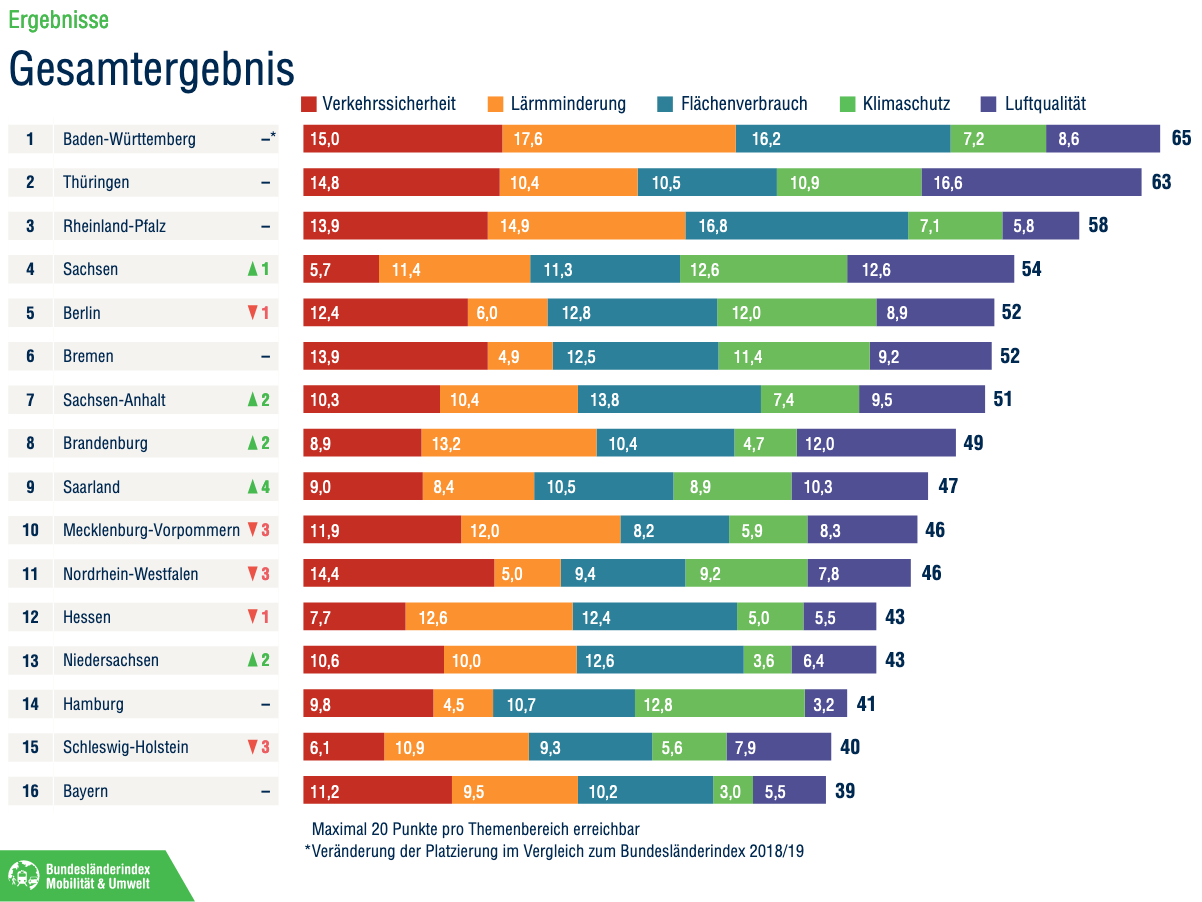
\includegraphics[width=14cm]{abbildungen/mob-index2020}
\centering
\caption[Bundesländerindex Mobilität \& Umwelt Ergebnisse]{Bundesländerindex Mobilität \& Umwelt Ergebnisse\footnotemark}
\label{mob-index2020}
\end{figure}
\footcitetext{Bundeslaenderindex:1}

Die Berechnung dees Bundesländerindex Mobilität basiert auf einer ausgeglichenen Gewichtung der betrachteten Faktoren.~\ref{mob-index2018-Verteilung})

\begin{figure}[H]
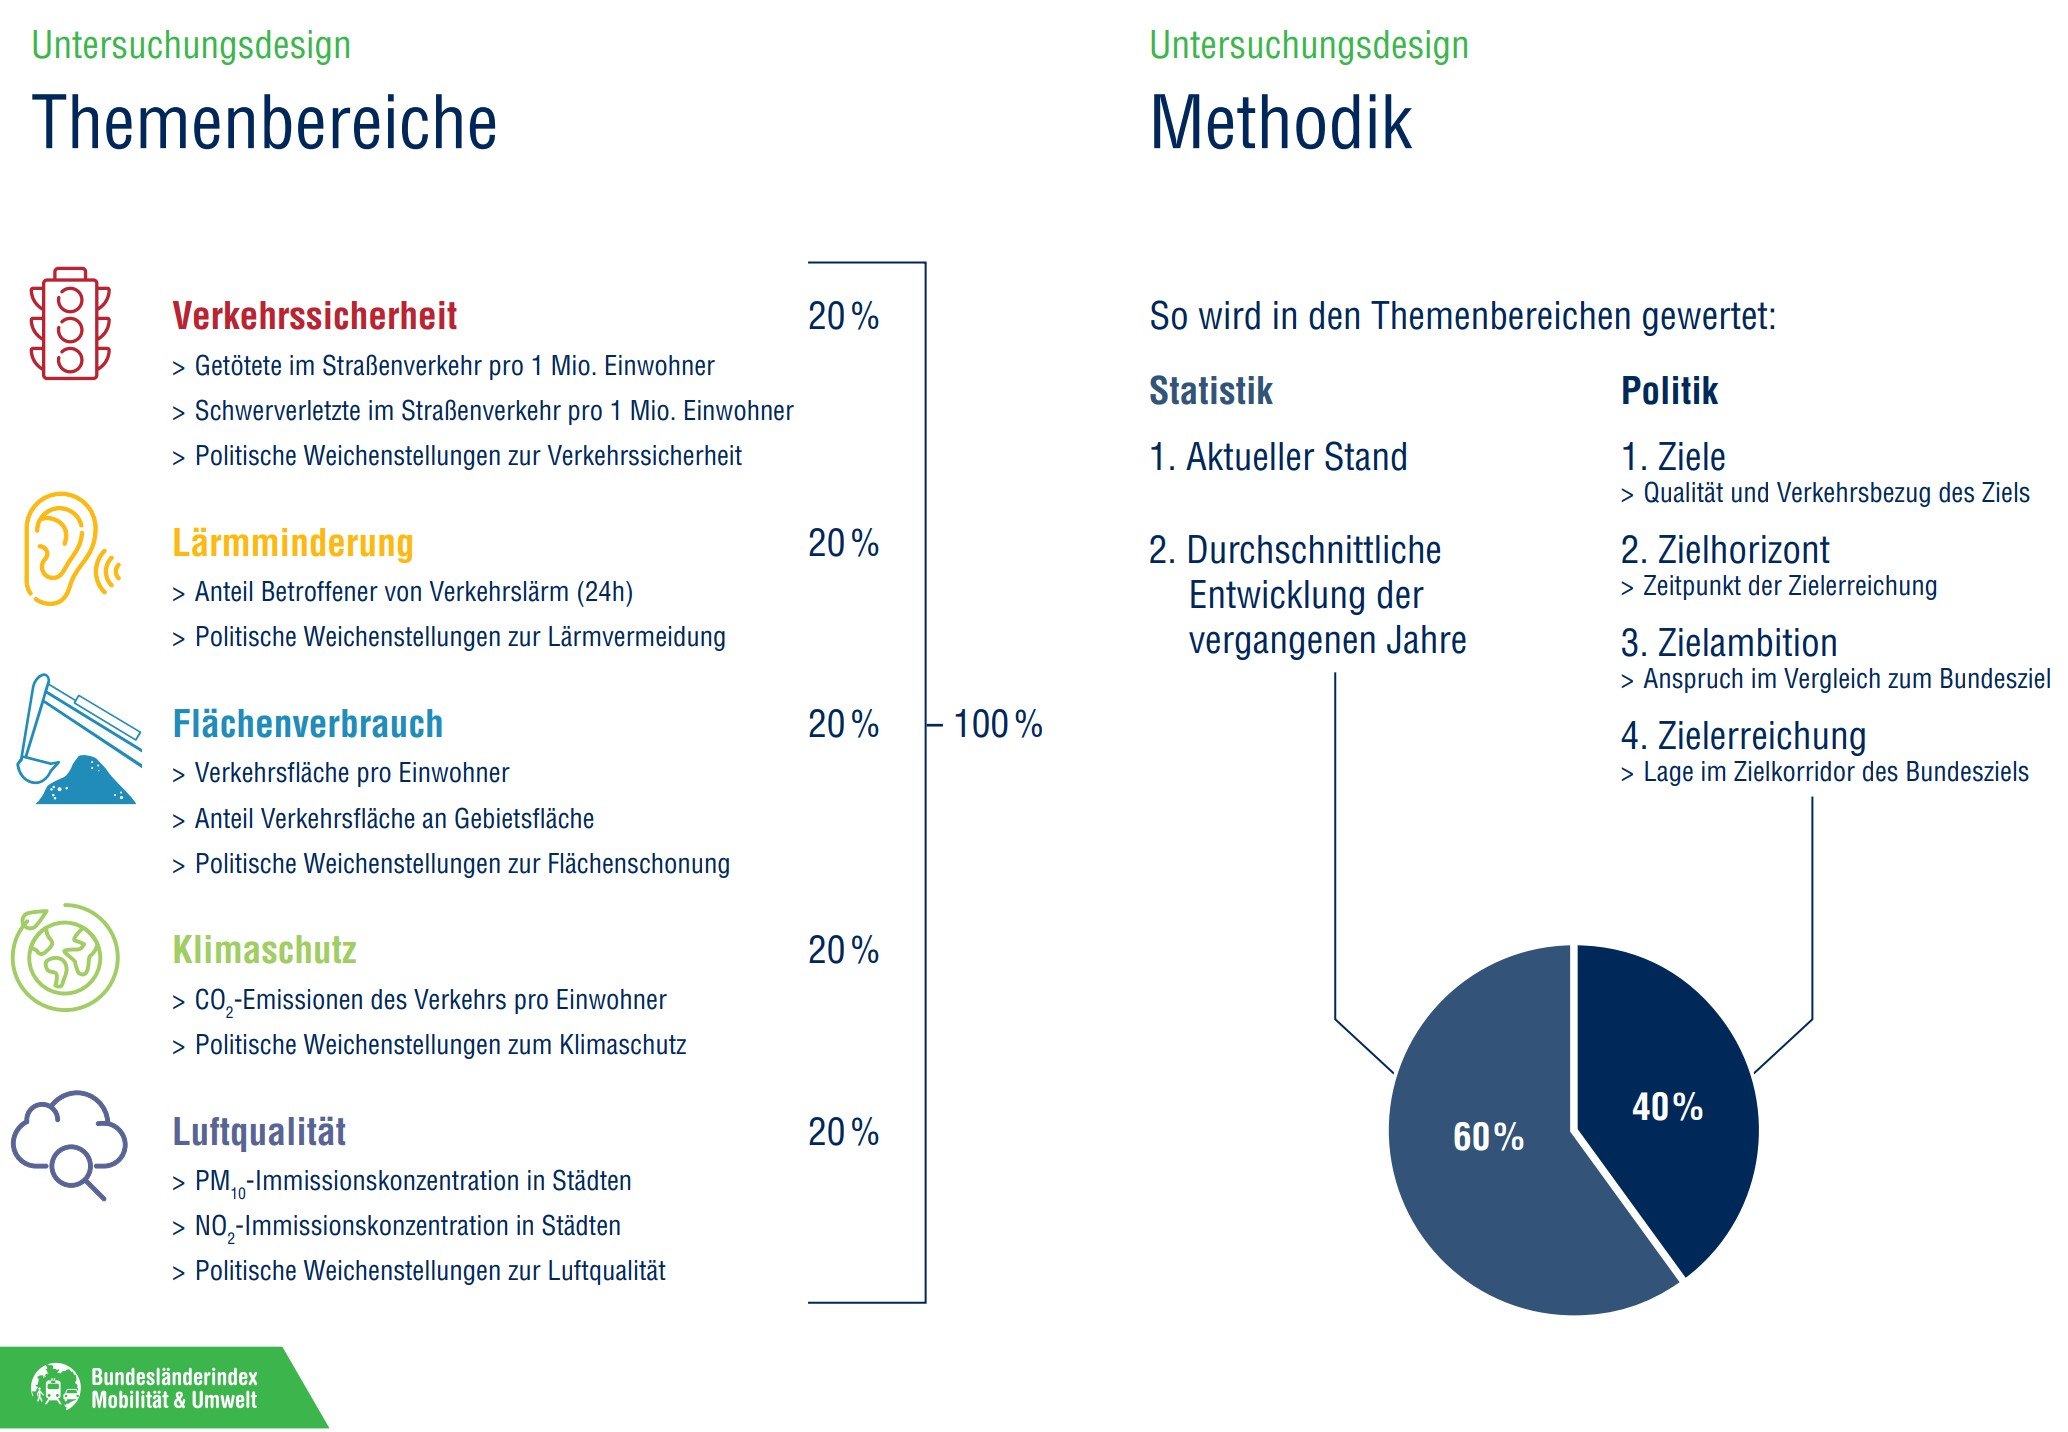
\includegraphics[width=14cm]{abbildungen/mob-index2018-Verteilung}
\centering
\caption[Bundesländerindex Mobilität \& Umwelt Gewichtung]{Bundesländerindex Mobilität \& Umwelt Gewichtung\footnotemark}
\label{mob-index2018-Verteilung}
\end{figure}
\footcitetext{Bundeslaenderindex:1}

Analog zum Bundesländerindex Mobilität \& Umwelt könnte ausgehend von den im vorliegendnen Bericht erarbeiteten Analyseansätzen ein Mobilitätsindex mit dem Schwerpunkt Anbindungsqualität entwickelt werden.  Ein solcher Mobilitätsindex würde ausgehend von der Analyse von Isochronen die Erreichbarkeit von Orten unter Berücksichtigung der ihrer Wichtigkeit darstellen. Durch eine Durch eine entsprechende Anreicherung der Datengrundlage könnte der Mobilitätsindex dahingehend ausgestaltet werden, dass der laufende Vergleich (Monitoring) der Anbindungsqualität auf Ebene von Bundesländern oder Städten möglich ist. Dieser Mobilitsindex mit dem Schwerpunkt Anbindungsqualität, könnte entweder gesondert entwickelt oder in den bestehenden Bundesländerindex Mobilität \& Umwelt integriert werden.



% Es wird dazu konstruktiv der folgende Vorschlag unterbreitet, der nur ein Minimum an Ergänzungen darstellt.

% \img{mob-index-anpassung}{mob-index-anpassung}{width=14cm}{Mobilitätsindex ergänzt und erweitert (eigene Darstellung)}

% Die in Abbildung~\ref{mob-index-anpassung} dargestellte Erweiterung sieht unter anderem eine andere Gewichtung vor. Vor allem sollten die genutzten Flächen einen höheren Beitrag zur Bewertung aufweisen. Dies könnte die Korrelation zwischen dicht besiedelten Gebieten und der Luftqualität abschwächen aber auch die CO2~Emittierung von dichten Industrieansiedlungen in dem Bundesland oder dem Stadtstaat.
% Am wichtigsten ist aber mitunter das Einführen einer neuen Datenquelle bzw. einer neuen Dimension. Der öffentliche Nahverkehr und der regionale Überlandverkehr ist besonders in nicht dicht besiedelten Gebieten essentiell.
% Das Abbilden des Ausbaus der Nutzung etc. zeigt in einem stetigen Mobilitätsindexes auch deren Entwicklung an und kann als Werkzeug zur Transparenz genutzt werden.
% Des Weiteren lassen sich mit einer immer komplexeren Formalisierung eines ganzheitlichen Indexes Städte, Bundesländer oder sogar Landkreise vergleichen. Dies ermöglicht Planer*innen aber auch Förderer*innen, Mittel und Maßnahmen an den geeigneten Stellen zu platzieren.
